\documentclass[a4paper,12pt]{article}
\usepackage[top = 2.5cm, bottom = 2.5cm, left = 2.5cm, right = 2.5cm]{geometry}
\usepackage[T1]{fontenc}
\usepackage[utf8]{inputenc}
\usepackage{multirow} 
\usepackage{booktabs} 
\usepackage{graphicx}
\usepackage[spanish]{babel}
\usepackage{setspace}
\setlength{\parindent}{0in}
\usepackage{float}
\usepackage{fancyhdr}
\usepackage{amsmath}
\usepackage{amssymb}
\usepackage{amsthm}
\usepackage[numbers]{natbib}
\newcommand\Mycite[1]{%
	\citeauthor{#1}~[\citeyear{#1}]}
\usepackage{graphicx}
\usepackage{subcaption}
\usepackage{booktabs}
\usepackage{etoolbox}
\usepackage{minibox}
\usepackage{hyperref}
\usepackage{xcolor}
\usepackage[skins]{tcolorbox}
%---------------------------

\newtcolorbox{cajita}[1][]{
	 #1
}

\newenvironment{sol}
{\renewcommand\qedsymbol{$\square$}\begin{proof}[\textbf{Solución.}]}
	{\end{proof}}

\newenvironment{dem}
{\renewcommand\qedsymbol{$\blacksquare$}\begin{proof}[\textbf{Demostración.}]}
	{\end{proof}}

\newtheorem{problema}{Problema}
\newtheorem{definicion}{Definición}
\newtheorem{ejemplo}{Ejemplo}
\newtheorem{teorema}{Teorema}
\newtheorem{corolario}{Corolario}[teorema]
\newtheorem{lema}[teorema]{Lema}
\newtheorem{prop}{Proposición}
\newtheorem*{nota}{\textbf{NOTA}}
\renewcommand\qedsymbol{$\blacksquare$}
\usepackage{svg}
\usepackage{pgfplots}
\pgfplotsset{compat=1.11}

\usepackage{tikz}
\usetikzlibrary{calc}

\usetikzlibrary{patterns}
\usepackage[framemethod=default]{mdframed}
\global\mdfdefinestyle{exampledefault}{%
linecolor=lightgray,linewidth=1pt,%
leftmargin=1cm,rightmargin=1cm,
}




\newenvironment{noter}[1]{%
\mdfsetup{%
frametitle={\tikz\node[fill=white,rectangle,inner sep=0pt,outer sep=0pt]{#1};},
frametitleaboveskip=-0.5\ht\strutbox,
frametitlealignment=\raggedright
}%
\begin{mdframed}[style=exampledefault]
}{\end{mdframed}}
\newcommand{\linea}{\noindent\rule{\textwidth}{3pt}}
\newcommand{\linita}{\noindent\rule{\textwidth}{1pt}}

\AtBeginEnvironment{align}{\setcounter{equation}{0}}
\pagestyle{fancy}

\fancyhf{}









%----------------------------------------------------------
\lhead{\footnotesize Geometría diferencial}
\rhead{\footnotesize  Rudik Roberto Rompich}
\cfoot{\footnotesize \thepage}


%--------------------------

\begin{document}
 \thispagestyle{empty} 
    \begin{tabular}{p{15.5cm}}
    \begin{tabbing}
    \textbf{Universidad del Valle de Guatemala} \\
    Departamento de Matemática\\
    Licenciatura en Matemática Aplicada\\\\
   \textbf{Estudiante:} Rudik Roberto Rompich\\
   \textbf{Correo:}  \href{mailto:rom19857@uvg.edu.gt}{rom19857@uvg.edu.gt}\\
   \textbf{Carné:} 19857
    \end{tabbing}
    \begin{center}
        Geometría diferencial - Catedrático: Alan Reyes\\
        \today
    \end{center}\\
    \hline
    \\
    \end{tabular} 
    \vspace*{0.3cm} 
    \begin{center} 
    {\Large \bf  Tarea
} 
        \vspace{2mm}
    \end{center}
    \vspace{0.4cm}
%--------------------------
\begin{cajita}
    Para responder esta pregunta, se tomó como referencia los siguientes modelos vistos en el curso, que se consideraron que ejemplifican bastante bien de forma resumida el contenido de todo el curso: 
    \begin{itemize}
        \item Modelo de media y varianza de Markowitz 
        \item CAPM
        \item BLM
        \item Modelos dinámicos no lineales, fractalidad y
        métodos cuánticos
        \item Movimiento Browniano (Procesos de Wiener)- Precio de acciones - Modelo Log-Normal del Precio de Mercado - Procesos y Lema de Ito 
        \item Precio de opciones call y put europeas - BSM
        \item Precios de opciones y productos financieros derivados (Letras griegas)
        \item Proyección de precios de commodities (Precios-Spot, modelo clásico básico) 
        \item Modelo forma reducida (Autoregresivos, Precios-Forward, Precios-Futuros)
        \item Proyección de precios de carteras de bonos (Precios de bonos, Carteras de bonos,Mapas de flujos de caja, Valor en riesgo) 
        \item Modelo forma estructural 

    \end{itemize}
\end{cajita}
\begin{problema}
    Exponga detalladamente de qué manera se relacionan cada uno de los modelos vistos en el curso con los nodos centrales de la teoría financiera clásica:
\begin{enumerate}
    \item Unidad del espacio de observación y medición
    \item Tiempo clásico
    \item Ausencia de interactividad entre el observador y el objeto
    \item Asociación entre eventos extremos y su relativa infrecuencia
\end{enumerate}

\begin{sol}
    Tenemos: 
    \begin{itemize}
        %----------
        \item Modelo de media y varianza de Markowitz.  Como se menciona en la guía, Markowitz es un modelo esencial para el CAPM, en donde es necesario examinar de qué manera la correlación imperfecta en los retornos de los activos financieros incide sobre el balance entre riesgo y retorno en la percepción del inversionista. 
        \begin{enumerate}
        \item \textbf{Unidad de la observación y el espacio de medición} Los inversionistas evalúan sus carteras de inversión según el retorno esperado y la desviación estándar del retorno, en un único horizonte/plazo de tiempo. Esto se relaciona con la unidad del espacio de observación y medición ya que el retorno esperado y la desviación estándar son las dos métricas clave en el modelo de Markowitz.
        \item \textbf{Tiempo clásico}
        El modelo de Markowitz se aplica a un único horizonte/plazo de tiempo, lo que se alinea con la noción de tiempo clásico.
        \item \textbf{Ausencia de interactividad entre el observador y el objeto}
        En el modelo de Markowitz, se asume que todos los inversionistas tienen acceso a las mismas oportunidades de inversión y comparten las mismas estimaciones de retornos esperados, desviaciones estándar y correlaciones entre activos de inversión. Esto sugiere una ausencia de interactividad entre el observador (el inversionista) y el objeto (el activo de inversión) 
        \item \textbf{Asociación entre eventos extremos y su relativa infrecuencia}
        El documento no proporciona información directa sobre cómo el modelo de Markowitz se relaciona con la asociación entre eventos extremos y su relativa infrecuencia. Sin embargo, el modelo de Markowitz se basa en la optimización de la cartera en función de la media y la varianza, lo que implica una consideración de la volatilidad y el riesgo, que pueden estar asociados con eventos extremos.
        \begin{figure}[H]
            \centering
            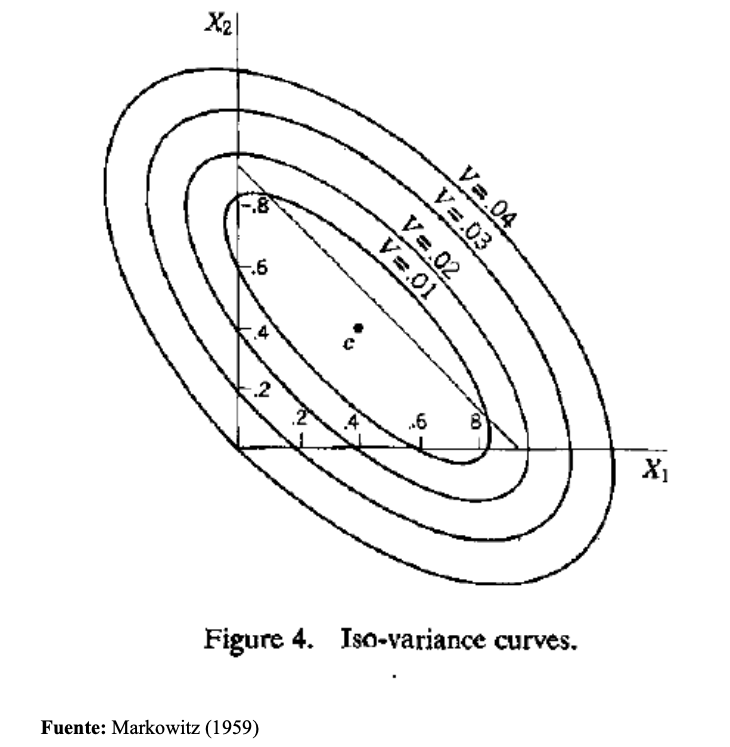
\includegraphics[scale=0.3]{imagenes/1.png}
        \end{figure}
        \end{enumerate}

        %---------    
        \item El Capital Asset Pricing Model (CAPM) es un modelo que describe la relación entre el riesgo sistemático de un activo individual (medido por su beta) y el rendimiento esperado de ese activo. Vamos a analizar cómo este modelo se relaciona con los nodos centrales de la teoría financiera clásica.

        \begin{enumerate}
        \item \textbf{Unidad de la observación y el espacio de medición}
        
        El CAPM se fundamenta en la observación y medición de ciertas variables. Para cada activo, necesitamos medir su rendimiento esperado, su rendimiento real y su beta, que es la medida de su riesgo sistemático. La fórmula del CAPM es la siguiente:
        
        \begin{equation*}
        E(R_i) = R_f + \beta_i \cdot (E(R_m) - R_f)
        \end{equation*}
        
        Donde:
        \begin{itemize}
        \item $E(R_i)$ es el rendimiento esperado del activo $i$,
        \item $R_f$ es el rendimiento libre de riesgo,
        \item $\beta_i$ es el coeficiente beta del activo $i$ (la medida de su riesgo sistemático), y
        \item $E(R_m)$ es el rendimiento esperado del mercado.
        \end{itemize}
        
        En donde cada una de las variables anteriores representan en conjunto la unidad de observación y espacio de medición. 
        
        \item \textbf{Tiempo clásico}
        
       Para responder esto, consideramos que el tiempo juega un papel crucial en el CAPM en dos aspectos principales. Siempre basándonos en la ecuación del inciso anterior. 

       \begin{itemize}
        \item La beta de un activo se calcula en basado de los rendimientos pasados, lo que podrías que implica una dependencia del tiempo.
        \item El rendimiento esperado de un activo se proyecta en el futuro, lo que también implica que está basado en el tiempo. Además, esto también hay que considerar  que el tiempo puede afectar al rendimiento libre de riesgo y al rendimiento del mercado.
       \end{itemize}
       
       
        \item \textbf{Ausencia de interactividad entre el observador y el objeto}
        
        En el CAPM, este nodo es bastante trivial. Ya que se asume que los inversores son tomadores de precios, lo que significa que sus decisiones individuales no pueden afectar a los precios de los activos. Esto implica directamente una ausencia de interactividad entre el observador (el inversor) y el objeto (el activo).
        
        \item \textbf{Asociación entre eventos extremos y su relativa infrecuencia}
        
        En el CAPM (en su versión elemental, la que vimos en el curso), no toma en cuenta directamente eventos extremos y su infrecuencia.\bigbreak 
        A pesar de esto, podríamos decir que en base a la beta de un activo, ya que podría ser interpretada como una medida del riesgo que el activo agrega a una cartera de mercado diversificada. Considerando esto, un activo con una beta alta podríua estar asociado con eventos extremos de alto rendimiento o de bajo rendimiento, aunque estos eventos sean infrecuentes.
        \end{enumerate}
        \item El modelo Black-Litterman (BLM) es un modelo que se basa en resolver las limitaciones y a los supuestos simplificados de modelos como el CAPM. En el contexto de los nodos centrales de la teoría financiera clásica, el BLM se relaciona de la siguiente manera:

        \begin{enumerate}
        \item \textbf{Unidad de la observación y el espacio de medida:}
        
        La teoría financiera clásica asume que los precios de los activos financieros siguen una distribución de probabilidad conocida, generalmente la normal. Sin embargo, en la práctica, los parámetros de estas distribuciones son inciertos. El BLM incorpora este hecho al introducir incertidumbre sobre los parámetros de la distribución de rendimientos. 
        
        La ecuación
        
        $$
        \mu = \pi + \varepsilon ;\quad \varepsilon \sim N\left(0, \Sigma_{\pi}\right)
        $$
        
        representa esta incertidumbre, con $\varepsilon$ como un término de error que sigue una distribución normal.
        
        \item \textbf{Tiempo clásico:}
        
        El BLM es un modelo que se aplica en un solo período de tiempo. Es decir que, se basa en la noción clásica de tiempo en la teoría financiera, el cual está basado en un solo período o como un número discreto de períodos.
        
        \item \textbf{Ausencia de interactividad entre el observador y el objeto:}
        
        Como en todos los modelos clásicos, en este modelo los inversionistas toman decisiones basadas en sus expectativas y de ninguna manera influyen en los precios de los activos. Sin embargo, también hay que considerar que el BLM permite cierta heterogeneidad (es decir, que no es tan rígido y permite la diversidad) en las creencias de los inversionistas, que es lo contrario a los supuestos de homogeneidad de modelos como el CAPM.
        
        \item \textbf{Asociación entre eventos extremos y su relativa infrecuencia:}
        
        El BLM no modela explícitamente los eventos extremos, porque básicamente se asume la normalidad de los rendimientos. Sin embargo, se podría decir que al incorporar incertidumbre sobre los parámetros de la distribución de rendimientos, el BLM permite cierta flexibilidad que podría utilizarse para dar cuenta de los eventos extremos.
        
        \end{enumerate}
        
    \item Modelos dinámicos no lineales, fractalidad y métodos cuánticos, en este apartado dejamos claro que los métodos cuánticos no son método como tal, sino que se hacen equivalencia entre conceptos financieros y ecuaciones físicas, por otra parte, también está la fractalidad, pero durante la clase únicamente se mencionó el concepto de la multifractalidad. Así que nos enfocaremos únicamente en los modelos no lineales.  Los Modelos Dinámicos No Lineales son útiles para describir comportamientos que no se pueden capturar adecuadamente con modelos lineales y la fractalidad:

    \begin{enumerate}
    \item \textbf{Unidad de la observación y el espacio de medición}
    
    En los Modelos Dinámicos No Lineales, las unidades de observación y medición pueden variar dependiendo del problema en cuestión. Aunque como en todos los modelos clásicos, estas unidades están relacionadas con variables financieras como precios de activos, rendimientos, volatilidad, entre otros. 
    \begin{itemize}
        \item Los modelos dinámicos no lineales pueden dar lugar a trayectorias de precios financieros muy complejas; estas trayectorias pueden sufrir grandes cambios, incluso de carácter cualitativo, como resultado de minúsculos cambios en algún factor del sistema. Esto se conoce como el "efecto mariposa", un ejemplo concreto es el atractor de Lorenz:
        \begin{figure}[H]
            \centering
            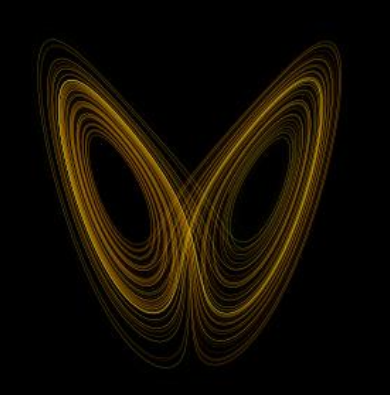
\includegraphics[scale=0.3]{imagenes/2.png}
        \end{figure}
    \end{itemize}
    
    
    \item \textbf{Tiempo clásico}
    
    El tiempo juega un papel central en los Modelos Dinámicos No Lineales. El tiempo en estos modelos se refleja en cómo las variables y los parámetros evolucionan a lo largo del tiempo. Además, estos modelos suelen incorporan "delays" que reflejan cómo los eventos pasados influyen en los eventos actuales y futuros.
    
    \item \textbf{Ausencia de interactividad entre el observador y el objeto}
    
    En su mayoría, los Modelos Dinámicos No Lineales asumen la ausencia de interactividad entre el observador y el objeto. Sin embargo, estos modelos son lo suficientemente flexibles como para ser extendidos para incluir formas de interacción, si es necesario para una aplicación específica.
    
    \item \textbf{Asociación entre eventos extremos y su relativa infrecuencia}
    
    Los Modelos Dinámicos No Lineales son útiles para modelar eventos extremos y su relativa infrecuencia. Estos modelos tienden a ser flexibles, lo que les permite capturar comportamientos como la asimetría, las colas pesadas y los cambios estructurales, que suelen estar asociados con eventos extremos en los datos financieros. Aunque para confirmarlo con certeza, habría que analizar un modelo en concreto. 
    \end{enumerate}

    %----------
\item Movimiento Browniano (Procesos de Wiener)- Precio de acciones - Modelo Log-Normal del Precio de Mercado - Procesos y Lema de Ito 
\begin{enumerate}
\item \textbf{Unidad de la observación y el espacio de medición}
Este modelo se basa en la variación $\Delta z$ durante un breve intervalo de tiempo $\Delta t$ esta dado por $\Delta z= \varepsilon \sqrt{\Delta t}$ donde $\varepsilon\sim \phi (0,1)$
\begin{itemize}
    \item Un ejemplo son el precio de las acciones que se modelan con un proceso de Wiener y se modela como $\Delta S= \mu S\Delta t$ al cual se le pude agregar un componente aleatorio $\sigma S dz$. 
    \item Otro ejemplo es el proceso de Ito, en su tiempo discreto que se modela como $\Delta x\approx a(x,y)\Delta t +b(x,t)\varepsilon \sqrt{\Delta t}$
\end{itemize}
\item \textbf{Tiempo clásico}
Los valores $\Delta r$ en dos intervalos breves de tiempo, $\Delta r$, son independientes. Esto implica que el proceso $\Delta r$ es un proceso de Markov.
\item \textbf{Ausencia de interactividad entre el observador y el objeto}
Como todos los modelos clásicos, en este modelo no se considera este aspecto. 
\item \textbf{Asociación entre eventos extremos y su relativa infrecuencia}
Este aspecto no se toma en cuenta, ya que $\varepsilon\sim \phi (0,1)$; y la distribución normal no considera eventos extremos. 
\end{enumerate}

%---------  

    \item El Modelo de Black-Scholes-Merton (BSM) es un modelo que se utiliza para valorar opciones financieras y derivados. El Modelo de Black-Scholes-Merton se relaciona con los nodos centrales de la teoría financiera clásica:

    \begin{enumerate}
    \item \textbf{Unidad de la observación y el espacio de medición}
    
    En el Modelo de Black-Scholes-Merton, la unidad de observación y medición es el precio de una opción. El modelo se basa en ciertas suposiciones para derivar una ecuación diferencial parcial que describe cómo cambia el precio de una opción con respecto al tiempo y al precio del activo subyacente. Por ejmplo, la ecuación Black-Scholes-Merton para una opción europea de compra es la siguiente:
    
    \begin{equation*}
    C(S, t) = S_tN(d_1) - Ke^{-r(T-t)}N(d_2)
    \end{equation*}
    
    Donde:
    \begin{itemize}
    \item $C(S, t)$ es el precio de la opción de compra,
    \item $S_t$ es el precio del activo subyacente en el tiempo $t$,
    \item $K$ es el precio de ejercicio de la opción,
    \item $r$ es la tasa de interés libre de riesgo,
    \item $T$ es el tiempo de vencimiento de la opción,
    \item $N(.)$ es la función de distribución acumulada de la distribución normal estándar, y
    \item $d_1$ y $d_2$ son dos términos que dependen de los demás parámetros.
    \end{itemize}
    
    \item \textbf{Tiempo clásico}
    
    El tiempo  es una parte esencial en el Modelo de Black-Scholes-Merton. El modelo considera cómo el precio de una opción cambia a medida que el tiempo avanza hacia la fecha de vencimiento de la opción. 
    
    \item \textbf{Ausencia de interactividad entre el observador y el objeto}
    
    El Modelo de Black-Scholes-Merton asume que los inversores son tomadores de precios, lo que implica una ausencia de interactividad entre el observador (el inversor) y el objeto (la opción). En otras palabras, las decisiones individuales de los inversores no afectan a los precios de las opciones en el mercado.
    
    \item \textbf{Asociación entre eventos extremos y su relativa infrecuencia}
    
    El Modelo de Black-Scholes-Merton asume que los rendimientos del activo subyacente siguen una distribución lognormal, lo que implica que el modelo no considera que sea significativo la probabilidad de eventos extremos.
\end{enumerate}

%----------
\item Precios de opciones y productos financieros derivados (Letras griegas)
\begin{enumerate}
\item \textbf{Unidad de la observación y el espacio de medición}
El Delta ($\Delta$) refleja el cambio en el precio del derivado con respecto a la fluctuación del precio del activo subyacente. El Delta no es constante, ya que la relación entre el precio de la opción y el precio subyacente no es exactamente lineal. Además, $\Gamma$ varía con el plazo al vencimiento

\item \textbf{Tiempo clásico}
Se conoce como theta ($\Theta$) al ritmo de cambio del valor de un producto o cartera financiera, con respecto al tiempo. Corresponde al tiempo de decaimiento, $\Theta= \partial \Pi/\partial t$. $\Theta$ no es constante, sino que depende del paso del tiempo y del precio subyacente
\item \textbf{Ausencia de interactividad entre el observador y el objeto}
Tiempo clásico, no hay interactividad. 
\item \textbf{Asociación entre eventos extremos y su relativa infrecuencia}
No se considera este aspecto, ya que no se consideran eventos extremos. 
\end{enumerate}

%---------  

%----------
\item Proyección de precios de commodities (Precios-Spot, modelo clásico básico) 
\begin{enumerate}
\item \textbf{Unidad de la observación y el espacio de medición}
Los commodities son productos físicos ampliamente comercializados en el mundo, como productos agrícolas, minerales o combustibles. Estos productos tienen una relativa homogeneidad, lo que significa que una vez establecidos determinados estándares técnicos, es sencillo determinar su cumplimiento.
\begin{itemize}
    \item Modelo clásico básico:
    $$D_t=D_t(P_t)=a-bP_t+u_t$$
    $$S_t=S_t(P_t)=\alpha +\beta P_t +v_t$$
\end{itemize}
\item \textbf{Tiempo clásico}
En el modelo clásico básico, se consideran choques aleatorios de oferta y demanda, pero sin inventarios ni rezagos en las respuestas. Esto implica que los precios de los commodities son altamente volátiles y están sujetos a factores como el clima, enfermedades, descubrimiento de nuevas fuentes, coyuntura política, terrorismo, entre otros. 
\item \textbf{Ausencia de interactividad entre el observador y el objeto}
La decisión de un productor no afecta directamente el precio del commodity, sino que este se determina por las condiciones del mercado. Entonces no está explícitamente expuesta la interactividad. 
\item \textbf{Asociación entre eventos extremos y su relativa infrecuencia}
Los precios de los commodities son altamente volátiles y están sujetos a choques aleatorios, por lo cual sí se consideran en sus modelos. Incluso hay una ecuación que modela la condición de equilibrio: 
$$D_t+\Delta I_t=S_t$$
\end{enumerate}

%--------- 

%----------
\item Modelo forma reducida (Autoregresivos, Precios-Forward, Precios-Futuros)
\begin{enumerate}
\item \textbf{Unidad de la observación y el espacio de medición}
Los modelos de forma reducida, como los autoregresivos, los precios forward y los precios futuros, sintetizan el comportamiento de los precios en el mercado, dejando implícitos los factores estructurales.
\begin{itemize}
    \item En autorregresivos, tenemos $$P_t = A\sum_{i=0}^{T-1} B^i +B^T P_{t-T}+C\sum_{i=0}^{T-1} B^i \varepsilon_{t-i}$$
    \item En precios-forward tenemos: 
    $$U(\tilde{\pi}_t)= E(\tilde{\pi}_t)-k\operatorname{Var}(\tilde{\pi}_t)$$
    \item En precios-futuros tenemos: 
    $$U(\tilde{\pi}_t)= E(\tilde{\pi}_t)-\frac{a}{2}\operatorname{Var}(\tilde{\pi}_t)$$
\end{itemize}

\item \textbf{Tiempo clásico}
Estos modelos tiene la ventaje que pueden calcularse de manera empírica, tanto en forma estructural y en forma reducida. Las formas estructurales tienden a relacionarse con  formas reducidas con el análisis de series temporales. 

\item \textbf{Ausencia de interactividad entre el observador y el objeto}
Como en todos los modelos, nunca se considera la interactividad entre el observador y el objeto. Aunque este caso, podríamos considerar  a la prueba de hipótesis nula ($H_0:B=1$) como una interacción, el cual se menciona el caso de los autorregresivos, pero es algo super empírico. 

\item \textbf{Asociación entre eventos extremos y su relativa infrecuencia}
No existe ninguna asociación, ni relación en estos modelos, ya que toman como referencia la varianza y la esperanza matemática, lo que directamente indica que usan una noción de distribución normal. 

\end{enumerate}

%--------- 

%----------
\item Proyección de precios de carteras de bonos (Precios de bonos, Carteras de
bonos, Mapas de flujos de caja, Valor en riesgo)
\begin{enumerate}
\item \textbf{Unidad de la observación y el espacio de medición}
La duración de un bono, el cual es el promedio ponderado del plazo en el que ocurrirán los flujos de caja asociados, se expresa en unidades de tiempo. Esto se relaciona con la unidad del espacio de observación y medición en la teoría financiera clásica.
\item \textbf{Tiempo clásico}
Los flujos de caja de los bonos son conocidos con certeza, es decir, no tenemos variables aleatorias. Esto se relaciona con el concepto de tiempo clásico en la teoría financiera, donde los eventos ocurren en un tiempo determinado. 
\item \textbf{Ausencia de interactividad entre el observador y el objeto}
La variación en la curva de rendimiento se asume como pequeña y paralela en todos los plazos, lo que permite obviar la ausencia de tasas de referencia confiables en ciertos plazos. Esto se relaciona con la ausencia de interactividad entre el observador y el objeto en la teoría financiera clásica, ya que las tasas de referencia no se encuentran disponibles en todos los plazos.
\item \textbf{Asociación entre eventos extremos y su relativa infrecuencia}
En el cálculo del Valor en Riesgo (VaR), se asume que las fluctuaciones de la curva de rendimiento de los bonos cupón cero son paralelas y pequeñas. Esto se relaciona con la asociación entre eventos extremos y su relativa infrecuencia en la teoría financiera clásica, ya que se asume que las variaciones extremas en la curva de rendimiento son infrecuentes.
$$\Delta Z\approx -ZD\Delta y $$
\end{enumerate}

%--------- 

%----------
\item Modelo forma estructural
\begin{enumerate}
\item \textbf{Unidad de la observación y el espacio de medición}
El modelo forma estructural desglosa con ecuaciones los principales factores que dan lugar a los precios. Un ejemplo que se menciona, es el modelo clásico prototipo que modela las funciones de oferta y demanda en el mercado. Esto implica que el modelo forma estructural proporciona una unidad de observación y medición al desglosar los factores que influyen en los precios.
\item \textbf{Tiempo clásico}
El modelo estructural supone que el incumplimiento puede darse únicamente al vencimiento y que conlleva la liquidación de la empresa, dejando por fuera la posibilidad de realizar reestructuraciones. Esto implica una concepción clásica del tiempo, en la que los eventos ocurren en momentos específicos y predecibles.
\item \textbf{Ausencia de interactividad entre el observador y el objeto}
El modelo estructural consiste de elementos básicos pero que tienen una gran repercusión. El modelo estadístico armoniza con otras facetas de la teoría financiera convencional. Esto sugiere que el modelo estructural se basa en la suposición de que no hay interacción entre el observador y el objeto de estudio. 
\item \textbf{Asociación entre eventos extremos y su relativa infrecuencia}
Como en todos los modelos clásicos, aquí no se consideran a los eventos extremos. 
\end{enumerate}

%--------- 


    \end{itemize}

        
\end{sol}

\end{problema}

\begin{problema}
    Empleando sus conocimientos de teoría cuántica, comente sobre las limitaciones de los modelos clásicos para explicar fenómenos como:
\begin{enumerate}
    \item Fluctuaciones en el nivel energético de los mercados (por ejemplo, volatilidad variable y
    cambios de régimen)
    \item Interactividad entre el mercado y los agentes que participan en él (por ejemplo, volatilidad
    implícita dependiente de la naturaleza de la interacción del agente con el mercado)
    \item Elevada frecuencia de eventos extremos y adversos (distribuciones sesgadas con exceso de
    curtosis y multimodalidad)
    \item El descuento del valor del dinero en el tiempo (el tiempo como dimensión anómala al
    compararse con otras dimensiones del mercado)
\end{enumerate}
\begin{sol}
    Tenemos: 
    \begin{cajita}
        Para responder esta pregunta, será necesario citar conceptos claves en la guía cuántico por lo que se colocará la página que se respalda cada ejemplo concreto.
    \end{cajita}
    
    \begin{enumerate}
    \item \textbf{Fluctuaciones en el nivel energético de los mercados}
    
    En el CAPM, el Modelo Black-Litterman y el BSM, se asume generalmente que la volatilidad es constante o determinada por factores sistemáticos. En los Modelos Dinámicos No Lineales, aunque se permite cierta variabilidad en la volatilidad, los cambios abruptos de régimen pueden ser difíciles de capturar. Como se vio a lo largo de la clase, los modelos clásicos asumen que el mercado sigue una distribución normal o un movimiento browniano geométrico, que no pueden capturar completamente las fluctuaciones. Por ejemplo, en el modelo BSM, que se da por

\begin{equation*}
dS_t = \mu S_t dt + \sigma S_t dW_t
\end{equation*}

en donde $\mu$ es el retorno esperado, $\sigma$ es la desviación estándar de los retornos (volatilidad), y $W_t$ es un proceso de Wiener. Se supone una distribución lognormal de los retornos con volatilidad constante, lo cual no suele ser el caso en los mercados del mundo real. Ahora bien, por otra parte, en los modelos cuánticos pueden representar estas fluctuaciones de manera más precisa utilizando el concepto de superposición cuántica y colapso de la función de onda. El estado del mercado podría representarse como un estado cuántico $|\Psi\rangle$, que es una superposición de diferentes estados de mercado (representados por los eigenestados $|i\rangle$).

\begin{equation*}
|\Psi\rangle = \sum_i c_i |i\rangle
\end{equation*}

Aquí, $c_i$ son las amplitudes para cada estado. Este estado evoluciona de acuerdo con la ecuación de Schrödinger,

\begin{equation*}
i\hbar \frac{d|\Psi\rangle}{dt} = H|\Psi\rangle
\end{equation*}

donde $H$ es el operador Hamiltoniano que representa la energía total del sistema. Esto permite modelar la volatilidad variable y los cambios de régimen como cambios en la energía potencial del sistema.


Para ser más específicos se consideran las siguientes limitaciones que se mencionan en la guía: 
\begin{itemize}
    \item Resistencia subjetiva al cambio: En los modelos clásicos, la resistencia subjetiva al cambio de compradores y vendedores juega un papel en determinar la brecha entre el centro de masa de probabilidad del precio y el precio en un equilibrio estructural clásico (página 185)
    \item Incertidumbre en los precios: La incertidumbre en torno a los precios observados desde la perspectiva cuántica difiere del error de medición clásico. En la teoría cuántica, la cantidad de información que transmite una transacción sobre el estado del mercado depende de la probabilidad de haber observado ese precio (página 185).
    \item Variaciones energéticas: En la teoría cuántica, no hay una implicación a partir de la ecuación de Schrödinger de que la relación entre el tiempo y la evolución de la amplitud probabilista tenga que ser constante. Las variaciones energéticas, que ocurren de manera cuantizada, provocan fluctuaciones en el ritmo de cambio de la función de onda con respecto al tiempo. Estas fluctuaciones energéticas están relacionadas con los cambios de régimen que se perciben en los mercados financieros (página 129).
    \item Relación no lineal entre los precios y la amplitud probabilista: En la teoría cuántica, la relación entre los precios y la amplitud probabilista no es una constante. Los aumentos de energía estarían vinculados con un alejamiento de la linealidad en la relación entre la función de onda y los precios. Este fenómeno puede estar relacionado con el fenómeno empírico de la “sonrisa de la volatilidad” (página 129).
\end{itemize}
    
    \item \textbf{Interactividad entre el mercado y los agentes que participan en él}
    
    El CAPM, el Modelo Black-Litterman y el BSM asumen que los inversores son tomadores de precios y no interactúan con el mercado. En los Modelos Dinámicos No Lineales, aunque los inversores pueden responder a los cambios en el mercado, no se modela explícitamente su influencia en los precios de los activos.\bigbreak
    
    Pero por su parte, la teoría cuántica, el efecto observador establece que únicamente por observar un sistema cuántico puede cambiar el estado del sistema. Esto se representa por un operador $M$ que actúa sobre el estado $|\Psi\rangle$, que lleva al colapso de la función de onda a un eigenestado particular, lo que podría interpretarse como la interactividad entre el mercado y los agentes que participan en él. 

    Para ser más específicos se consideran las siguientes limitaciones que se mencionan en la guía: 
    \begin{itemize}
        \item Flexibilidad limitada: Aunque los modelos clásicos pueden adaptarse para incorporar factores como las distribuciones de dividendos, las variaciones de las tasas de retorno, o la posibilidad de cambios aleatorios de régimen, estas adaptaciones pueden ser complejas y no siempre son prácticas. Además, los modelos clásicos pueden tener dificultades para incorporar situaciones excepcionales en los procesos de precios, como una distribución de dividendos o la posibilidad de realizar el ejercicio temprano de una opción (página 212 y 214).
        \item Resistencia subjetiva al cambio: Los modelos clásicos pueden no tener en cuenta la resistencia subjetiva al cambio de los compradores y vendedores, que puede jugar un papel en determinar la brecha entre el centro de masa de probabilidad del precio y el precio en un equilibrio estructural clásico (página 185).
    \end{itemize}
    
    \item \textbf{Elevada frecuencia de eventos extremos y adversos}
    
    El CAPM y el BSM, que asumen que los rendimientos de los activos siguen una distribución normal, subestiman la probabilidad de eventos extremos. Aunque el Modelo Black-Litterman y los Modelos Dinámicos No Lineales permiten cierta flexibilidad en la distribución de los rendimientos, pueden no capturar plenamente las distribuciones sesgadas con exceso de curtosis y multimodalidad.\bigbreak
    
    Como ejemplo, en el modelo BSM y otros modelos clásicos suponen una distribución lognormal de los retornos con varianza finita, lo que no permite la ocurrencia de eventos extremos con alta frecuencia. Sin embargo, en los modelos cuánticos se puede modelar esto con la incertidumbre cuántica y permitiendo un rango más amplio de posibles resultados y esto se modela por el principio de incertidumbre de Heisenberg,


    \begin{equation*}
    \Delta x \Delta p \geq \frac{\hbar}{2}
    \end{equation*}
    
    que establece que hay un límite fundamental a la precisión con la que los pares de propiedades físicas de una partícula, como la posición $x$ y el momentum $p$, pueden ser conocidas simultáneamente.
    
    Para ser más específicos se consideran las siguientes limitaciones que se mencionan en la guía: 
    \begin{itemize}
        \item Límite al conocimiento obtenible: En el paradigma cuántico, hay un límite al conocimiento que puede obtenerse de un objeto cuántico a través de la observación. Esto contrasta con el optimismo del paradigma clásico y sugiere que las exigencias epistémicas para que los métodos clásicos sean aplicables son mayores (página 11).
        \item Interdependencia de eventos: En el caso de los objetos cuánticos, los eventos no pueden necesariamente tratarse como independientes para el cálculo de las probabilidades. Esto requiere un enfoque diferente, como la formulación integral de trayectorias de Feynman, que suma todas las trayectorias posibles, incluyendo las de interferencia (página 46).
    \end{itemize}

    \item \textbf{El descuento del valor del dinero en el tiempo}
    
    En el CAPM, el Modelo Black-Litterman, los Modelos Dinámicos No Lineales y el BSM, el tiempo es tratado como una dimensión continua y homogénea. Sin embargo, en la práctica, el tiempo puede ser percibido y experimentado de manera diferente por diferentes inversores y puede tener efectos variables en diferentes activos. Si embargo, por otra parte, en la teoría cuántica, el tiempo puede ser tratado con igualdad con las dimensiones espaciales.\bigbreak

    Por ejemplo, en la integral de camino de Feynman de la mecánica cuántica, la amplitud para que una partícula vaya del punto $A$ al punto $B$ se da por una suma sobre todos los caminos posibles, cada uno pesado por un factor de fase $e^{iS/\hbar}$, donde $S$ es la acción a lo largo del camino. Esto permite la consideración de todos los posibles caminos a través del tiempo, que podría ser una forma de modelar el valor del dinero en el tiempo de una manera más matizada.

    Para ser más específicos se consideran las siguientes limitaciones que se mencionan en la guía: 

    \begin{itemize}
        \item Origen del descuento: Los modelos clásicos aportan pocas luces en cuanto al origen de ese descuento. En contraste, un ajuste de los estados futuros del mercado emerge con naturalidad a partir del propagador cuántico y la ecuación de Schrödinger, como un resultado integrado en las funciones de amplitud probabilista que se desprenden de la evolución del estado del mercado (página 158).
        \item Incertidumbre: En ausencia de incertidumbre, el precio seguiría un proceso de composición continua a la tasa $\mu$, no muy diferente al que usaríamos para describir un instrumento con un rendimiento fijo y composición continua. Sin embargo, la incertidumbre es una característica central del comportamiento de las acciones (página 206).
        \item En términos de ecuaciones matemáticas, podemos ver que el descuento del valor del dinero en el tiempo se puede expresar en términos cuánticos como:
        
        $$\langle x'|\exp\left[\frac{iH}{r\hbar} (-rT)\right] |x \rangle$$
        
        Donde $x'$ es el logaritmo del precio futuro, $x$ es el logaritmo del precio presente, $H$ es el operador Hamiltoniano, $\hbar$ es la constante de Planck reducida y $r$ es la tasa de descuento arbitraria. (Página 159).
    \end{itemize}
    \end{enumerate}
    De esto, se resume con la siguiente tabla:
    \begin{table}[h]
        \centering
        \resizebox{\columnwidth}{!}{%
        \begin{tabular}{|l|p{5cm}|p{5cm}|}
        \hline
        \textbf{Fenómeno} & \textbf{Limitaciones de los Modelos Clásicos} & \textbf{Perspectiva Cuántica} \\
        \hline
        Fluctuaciones en el nivel energético de los mercados & Supone que la volatilidad es constante o determinada por factores sistemáticos. Difícil de capturar cambios abruptos de régimen. & Utiliza superposición cuántica y colapso de la función de onda para representar fluctuaciones con precisión. \\
        \hline
        Interactividad entre el mercado y los agentes que participan en él & Supone que los inversores son tomadores de precios y no interactúan con el mercado. & Aplica el efecto observador, indicando que la observación de un sistema cuántico puede cambiar su estado. \\
        \hline
        Elevada frecuencia de eventos extremos y adversos & Asume que los rendimientos de los activos siguen una distribución normal, subestimando la probabilidad de eventos extremos. & Utiliza la incertidumbre cuántica, permitiendo un rango más amplio de posibles resultados. \\
        \hline
        El descuento del valor del dinero en el tiempo & Trata el tiempo como una dimensión continua y homogénea, pudiendo ser percibido y experimentado de manera diferente por diferentes inversores. & Trata el tiempo en pie de igualdad con las dimensiones espaciales, permitiendo considerar todos los posibles caminos a través del tiempo. \\
        \hline
        \end{tabular}}
        
        \end{table}
        
\end{sol}
\end{problema}


%---------------------------
%\bibliographystyle{apa}
%\bibliography{referencias.bib}

\end{document}